\chapter{Background}

\section{The Semantic Web - A Web with a meaning} 
The Semantic Web is a collaborative movement led by W3C\footnote{The international standards body, the World Wide Web Consortium (W3C)} that promotes common data formats on the world wide web by encouraging semantic content in web pages. W3C's "Semantic Web Vision" is a future where: 
\begin{itemize}
\item Web information has exact meaning
\item Web information can be understood and processed by computers
\item Computers can integrate information from the web 
\end{itemize}

Natural languages have ambiguous meanings and even
a human reader may in some cases have problems understanding the correct
meaning of a text. If someone ask me  "Do you know Zlatan?" they may refer to if I know him as a friend or if Iknow who he is. It is the same for computers when they are trying to understand the meaning of a text. By adding labels to the text we can make it easier to interpret and thus creating a semantic web, formed so that software can collect and analyze data. The aim is that system can present the answer to a query instead of a page where the answer can be found, and answer queries where the answer is spread over several documents.
The semantic web is a web of data, where the data can be stored in documents in various ways. Using RDF is a way to structure data, so that it can be linked to other data with information and realations to objects.

\subsection{RDF}
Resource Description Framwork (RDF) is a general method to describe or model information that is implemented in web resources. It is based upon the idea of making statements about resources in the form of triples of subject-predicate-object. The subject denotes the resource (it can be anything that can have a URI), the predicate denotes traits or aspects of the resource and also expresses a relationship between the subject and the object. For example: "The sky" (subject) "has the color" (predicate) "blue" (object) could be an RDF triple.\\\\
Let's take a look at an example\footnote{Full example can be viewed at \url{http://www.w3schools.com/rdf/rdf_example.asp}} of an RDF object describing two CDs.\\
\begin{minted}[bgcolor=bg, label=XML example]{xml}
<?xml version="1.0"?>
<rdf:RDF 
  xmlns:rdf="http://www.w3.org/1999/02/22-rdf-syntax-ns#"
  xmlns:cd="http://www.recshop.fake/cd#"/>

  <rdf:Description
  rdf:about="http://www.recshop.fake/cd/Empire Burlesque"/>
    <cd:artist>Bob Dylan</cd:artist>
    <cd:country>USA</cd:country>
    <cd:company>Columbia</cd:company>
    <cd:price>10.90</cd:price>
    <cd:year>1985</cd:year>
  </rdf:Description>

  <rdf:Description
  rdf:about="http://www.recshop.fake/cd/Hide your heart"/>
    <cd:artist>Bonnie Tyler</cd:artist>
    <cd:country>UK</cd:country>
    <cd:company>CBS Records</cd:company>
    <cd:price>9.90</cd:price>
    <cd:year>1988</cd:year>
  </rdf:Description>
</rdf:RDF>
\end{minted}
\linebreak
\newline
The two lines at the top, \textbf{xmlns:rdf} and \textbf{xmlns:cd} define from which namespace elements with the rdf and cd prefix are from. The \textbf{rdf:Description} element contains the description of the resource identified by the \textbf{rdf:about} attribute. Finally the elements \textbf{cd:artist, cd:country, cd:company} etc. are properties of the resource.

\section{RDFa}
RDFa is a syntax for embedding an RDF graph in an XHTML document by using XHTML attributes for expressing RDF properties. It was proposed by Mark Birbeck in the form of a W3C note entitled XHTML and RDF\footnote{Bibliography [2] "XHTML and RDF W3C Note 14 February 2004". World Wide Web Consortium. 2004-02-14. Retrieved 2007-12-27.}.\\\\
RDFa is based on attributes that are used to carry metadata in an XML/HTML/XHTML language. There are some attributes that have been reused, for example “href” and “src” that comes from the HTML syntax. Then there is also a set of new attributes that are specified for RDFa, the attributes are: 
\begin{itemize}
\item \textbf{about} - A URI specifying the resource the metadata is about
\item \textbf{rel and rev} - A relationship and reverse-relationship with another resource, respectively
\item \textbf{src, href and resource} - The partner resource
\item \textbf{property} - A property for the content
\item \textbf{content} - optional attribute that overrides the content of the element when using the property attribute
\item \textbf{datatype} - optional attribute that specifies the datatype of text specified for use with the property attribute
\item \textbf{typeof} - optional attribute that specifies the RDF type(s) of the subject or the partner resource
\end{itemize}
Not all (X)HTML validators recognize and know how to validate these attributes, however this is usually not a problem when using a browser to view the document since most browsers ignore attributes that they not recognize. This means that the RDFa attributes does not have any effect on what is displayed to the user.\\\\
Below we have a simple example\footnote{For more RDFa examples see \url{http://en.wikipedia.org/wiki/RDFa}} where RDFa is used to markup basic information about a book. Here we are using Dublin Core to add metadata to this document, it is declared at the top so later on in the text we can use the prefix “dc” followed by the Dublin Core data element for the element we are describing (for example title).\\  
\begin{minted}[bgcolor=bg]{html}
<div xmlns:dc="http://purl.org/dc/elements/1.1/"
  about="http://www.example.com/books/wikinomics">
  <span property="dc:title">Wikinomics</span>
  <span property="dc:creator">Don Tapscott</span>
  <span property="dc:date">2006-10-01</span>
</div>
\end{minted}
\linebreak
\newline
Essentially what we are trying to do is to bridge the gap between what the computer sees and what a human reader sees. Giving the computer a way to know that headline expresses a title or that the sub-headline indicates the author, hints that a human reader understands while the computer only sees headline and sub-headline. 

\section{Linked Data - Connect data across the Web}
The Semantic Web isn't just about putting data on the web. It is about creating connections through links, so that when you have some of it, you can find other, related, data.\\\\
The term Linked data describes a method of publishing structured data so that it can be interlinked and become more useful. This is done by following a data model which is based on resources and that describe their properties, including relationships to other resources. By using standardized names for resources and property types, data sets from many different providers integrated. By expressing the relationships between resources in different data sets, a user may discover additional relevant data.\\
The foundation of linked data are the technologies HTTP and URIs. Today we use them (and many other services) to present human readers with web pages, linked data extends this to share information in a way that can be read, connected and queried automatically by computers. This is as a concept is not new, and have been used in other similar situations such as database network models and headings in library catalogs.\\\\
Tim Berners-Lee,\footnote{TODO: add src on Tim} the father of the World Wide Web coined the term \textit{“Linked Data”} and outlined four principles of linked data:
\begin{enumerate}
\item{Use URIs to identify things.}
\item{Use HTTP URIs so that these things can be referred to and looked up ("dereferenced") by people and user agents.}
\item{Provide useful information about the thing when its URI is dereferenced, using standard formats such as RDF/XML.}
\item{Include links to other, related URIs in the exposed data to improve discovery of other related information on the Web.}
\end{enumerate}
A community project called \textit{Linking Open Data\footnote{WC3 Semantic Web Education and Outreach group's - Linking Open Data community project}}, organized by W3C aims to extend the Web by publishing various open datasets as RDF on the Web by creating RDF links between data items from different data sources. In October 2007, the datasets consisted of over two billion\footnote{TODO: Add src} RDF triples, which were interlinked by over two million RDF links. By September 2011 this had grown to 31 billion RDF triples, interlinked by around 504 million RDF links.\\\\
The image below shows datasets that have been published in Linked Data format, by contributors to the Linking Open Data community project and other individuals and organizations. The purpose of this image is merely to depict the extent of such a project, not to present the details of the data sets.\footnote{See \url{http://lod-cloud.net/} for a more detailed image with links to all the contributors.}
\begin{center}
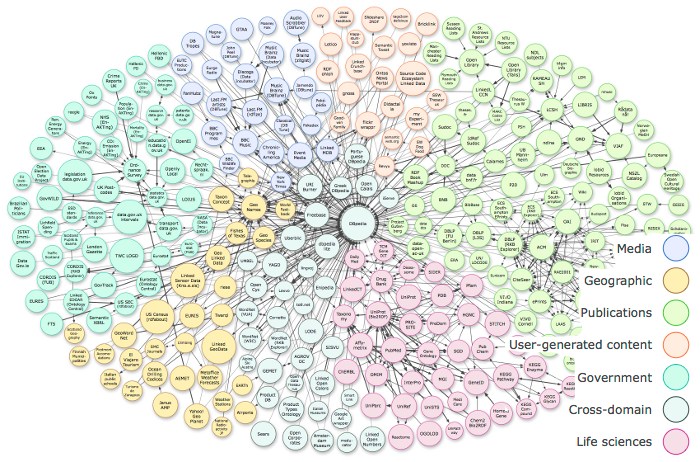
\includegraphics[scale=0.6]{../imgs/lod-datasets.png}
\captionof{figure}{Linking Open Data cloud diagram, by Richard Cyganiak and Anja Jentzsch.}
\end{center}

\section{Swedish law}
The main legislative powers are the parliament (Riksdagen) and the government (Regeringen), these institutions can adopt statutes which are published in the main official collection of statutory law, the \textit{Svensk Författningssamling} (SFS). The statutes enacted by the parliament are referred to as laws, and the statutes enacted by the government as ordinances.\\\\
When a statute is changed, this is done by adopting a new statute (the change statute) that states what sections of the old statute (the base statute) are to be changed, and how. There is not a new merged version published of the statute in SFS, only the base statute and change statute(s).\\\\
Two recurring definitions in this paper are legal sources and legal source documents. A legal source is a type of legal information such as a constitution in SFS or verdicts from one of the Swedish courts. A legal source document is a specific document for a certain legal source, such as \textit{Personuppgiftslagen} (SFS 1998:204). 
\subsection{Law structure}
Today there's 3000 constitutions but there's no well defined structure that describes how a law should look like. One thing that is common is that each law has an SFS number, including legislations amending already existing laws. The SFS number consists of a four digit year, a colon and a serial number assigned in chronological order of the date of issue. 

\subsection{Rättsinformationssystemet}
\textit{Rättsinformationssystemet} is the state's system to make legal information such as laws, legislative histories, court cases, etc. - available to the public via the Internet. This information is produced by a number of different authorities. Today, each agency is responsible for publishing "their" information via their own website. It is all tied together by the website \url{http://www.lagrummet.se} which is referring to each agency's respective legal information page.\\
This decentralized approach has its advantages. It gives the authorities a lot of freedom to design their information in a way that fits them. A downside is that they use this freedom to invent their own standards. \textit{Rättsinformationsförordningen}\footnote{Rättsinformationssystemet is regulated in this ordinance (1999:175)} is not very detailed on how the information should be presented, only that it should be published.\\\\
An additional purpose with the system is the ability for the private sector to re-use government information to create added value services\footnote{Services like Rättsnätet from Notisum and lagen.nu}. Legal information is of great value, that could be even better utilized if it was easier to re-use the information.
